%%%%%%%%%%%%%%%%%% USAGE INSTRUCTIONS %%%%%%%%%%%%%%%%%%
% - Compile using LuaLaTeX and biber, unless there is a particular reason not to. Do not use the older LaTex/PDFLaTeX or BibTeX. (The fonts won't work correctly.)
% - Font and the report 'year' must be specified when all \documentclass or the template won't work correctly. (There's no error checking/default cases!)
% - For best performance save images/graphics as PDF files, not as png/jpg/eps. This makes no difference to how images are inserted using \includegraphics.
% - As many further packages as wanted can be loaded. Below are just an example set. Note that template itself loads a number of packages, including hyperref.
% - References are handed using biblatex.
% - Link to the presentation of theses policy: https://documents.manchester.ac.uk/DocuInfo.aspx?DocID=2863



%%%%%%%%%%%%%%%%%% META DATA SETUP %%%%%%%%%%%%%%%%%%
% This is where the document title and author are set. Other details for the title page are set later
\begin{filecontents*}{\jobname.xmpdata}
  \Title{Third Year Project Report - Blood Glucose Forecasting using Machine Learning} 
  \Author{10444901} % should be student number rather than name to help with annoymous marking
  \Language{en-GB}
  \Copyrighted{True}
  % More meta-data fielda can be added here if wanted, see https://ctan.org/pkg/pdfx?lang=en for fields
\end{filecontents*}


%%%%%%%%%%%%%%%%%% DOCUMENT SETUP %%%%%%%%%%%%%%%%%%
\documentclass[times,thesis]{uom_eee_dissertation_casson} 



%%%%%%%%%%%%%%%%%% PACKAGES AND COMMANDS %%%%%%%%%%%%%%%%%%

% Packages
\usepackage{graphicx,psfrag,color} % for postscript graphics files
  \graphicspath{ {./images/} }
\usepackage{amsmath}               % assumes amsmath package installed
  \allowdisplaybreaks[1]           % allow eqnarrays to break across pages
\usepackage{amssymb}               % assumes amsmath package installed 
\usepackage{url}                   % format hyperlinks correctly
\usepackage{rotating}              % allow portrait figures and tables
\usepackage{multirow}              % allows merging of rows in tables
\usepackage{lscape}                % allows pages to be typeset in landscape mode
\usepackage{tabularx}              % allows fixed width tables
\usepackage{verbatim}              % enhanced version of built-in verbatim environment
\usepackage{footnote}              % allows more control over footnote environments
\usepackage{float}                 % allows H option on floats to force here placement
\usepackage{booktabs}              % improve table line spacing
\usepackage{lipsum}                % for adding dummy text here
\usepackage{subcaption}            % for multiple sub-figures in a single float
% Add your packages here

% Optional: for adding alt-text to images:
%\usepackage{pdfcomment}            % for alt text for accessibility
% Then to add images use:
% \pdftooltip{\includegraphics[width=0.5\textwidth]{image.pdf}}{Alt-text here}
% This makes the text in the image non-select-able though (assuming it's a vector file)

% Custom commands
\newcommand{\degree}{\ensuremath{^\circ}}
\newcommand{\sus}[1]{$^{\mbox{\scriptsize #1}}$} % superscript in text (e.g. 1st)
\newcommand{\sub}[1]{$_{\mbox{\scriptsize #1}}$} % subscript in text
\newcommand{\sect}[1]{Section~\ref{#1}}
\newcommand{\fig}[1]{Fig.~\ref{#1}}
\newcommand{\tab}[1]{Table~\ref{#1}}
\newcommand{\equ}[1]{(\ref{#1})}
\newcommand{\appx}[1]{Appendix~\ref{#1}}



%%%%%%%%%%%%%%%%%% REFERENCES SETUP %%%%%%%%%%%%%%%%%%

% Setup your references here. Change the reference style here if wanted
\usepackage[style=ieee,backend=biber,backref=true,hyperref=auto]{biblatex}
% Note backref=true adds a page number (and hyperlink) to each reference so you can easily go back from the references to the main document. You may prefer backref=false if you need to stick strictly to a given reference style


% Fixes which can't be applied in the .cls file
\DefineBibliographyStrings{english}{backrefpage = {cited on p\adddot},  backrefpages = {cited on pp\adddot}}
  \renewcommand*{\bibfont}{\large}


% Add more .bib files here if wanted
\addbibresource{references.bib}



%%%%%%%%%%%%%%%%%% START DOCUMENT %%%%%%%%%%%%%%%%%%

% Don't edit these lines, title and author are automatically taken from the document meta-data defined above
\begin{document}
\makeatletter
\title{Third Year Project Report - Blood Glucose Forecasting using Machine Learning}
\studentid{10444901}
\makeatother

% Set the below yourself
\course{Computer Science}  % "Master of Science in" is added automatically
                                                   
\submitdate{2023}                                  % regulations ask only for the year, not month
\wordcount{10000}		                           % use \wordcount{} to set the count, \thewordcount to print in the text
\maketitle


%%%%%%%%%%%%%%%%%% LISTS OF CONTENT %%%%%%%%%%%%%%%%%%
\uomtoc% other lists are not required, but can include \uomlof and \uomlot if really want to


%%%%%%%%%%%%%%%%%% ABSTRACT %%%%%%%%%%%%%%%%%%
\begin{abstract} % put abstract here. Limit is 1 page.
  This is abstract text. 
  
\end{abstract}%
\clearpage

%%%%%%%%%%%%%%%%%% SECTION 1 %%%%%%%%%%%%%%%%%%
\section{Introduction}

  \subsection{Background and motivation}
    Talk about diabetes generally, can take from introduction of lit review

    Type 1 Diabetes Mellitus (T1DM) is a life-long autoimmune disease that typically manifests itself in children between 10 and 14 years of age. That is not to say, however, that a diagnosis of T1DM is restricted to those individuals within this age range, and whilst it is rare for diagnosis to be made in individuals over 40, it is possible for a diagnosis of T1DM to occur at any age. T1DM is characterised by the destruction of the beta-cells within the pancreas which are responsible for producing insulin \cite{t1d}, a hormone used  by the body to help blood glucose to be absorbed by cells to be used for energy \cite{insulin}, and to store blood glucose for later use. This loss of insulin producing beta cells means that there is an inability for T1DM patients to regulate their own blood glucose levels, which if left untreated can lead to hyperglycemia (blood glucose levels being too high). As such, T1DM patients are reliant on the subcutaneous injection of synthetic insulin to control the glycemic levels in their body and to maintain a healthy blood glucose level. Diagnosis of the condition is based on hyperglycemia, with a fasting blood glucose concentration above 7.0 mmol/L being characterised as enough to diagnose. Other symptoms commonly seen before diagnosis are going to the toilet a lot, constantly being thirsty, and weight loss \cite{t1dcauses}.

    In order to calculate how much external insulin to inject, and thus avoid hyperglycemia and hypoglycemia (blood glucose levels being too low), T1DM patients must keep track of how much glucose they ingest and dose themselves with a corresponding volume of insulin. This counting and dosing process is not an exact science, and being inaccurate can lead to potentially life-threatening situations for patients. As such, technology has been introduced to make the process easier. Continuous Glucose Monitoring (CGM) devices \cite{pumpcgm} provide real-time information on someone's current Blood Glucose (BG) levels, whilst insulin pumps exist that are capable of slowly providing insulin over a long period of time, rather than having a single large dose given by injection pen. This new technology has greatly improved the lives of many patients, and there is hope that new technology can continue to do the same. One of the main issues with current technology is that whilst it is able to immediately detect issues with current BG levels, there is still a response time between corrective actions being taken and their impacts on BG levels. This response time has lead to much research being done into predictive algorithms that could inform a patient ahead of time of any issues that may occur, allowing them to react with ample time and avoid any high/low blood glucose levels before they even manifest. One such branch of these predictive algorithms is machine learning algorithms and an exploration of this topic will form the basis of this project report.
  
  \subsection{Aims and objectives}
    This project aims to investigate and implement machine learning methods to perform blood glucose prediction, then compare and contrast the performance of these different methods.

    To guide the development of the project, the following objectives have been identified: 
    \begin{itemize}
        \item Obtain, understand and configure a suitable Continuous Glucose Monitoring (CGM) dataset.
        \item Perform a literature review on existing approaches taken to perform blood glucose prediction.
        \item Implement a selection of the researched approaches.
        \item Experiment with hyperparameters on different approaches to try and achieve optimal accuracy for the approach as stated by scientific metrics.
        \item Experiment with the different approaches over varying prediction horizons.
        \item Produce visualisations to view the performance of the different prediction techniques over differing time horizons.
        \item Analyse and compare the effectiveness of the different approaches blood glucose prediction.
        \item Discuss the work that would need to be done to make such prediction technologies available and useful to real patients.
    \end{itemize}
    
  \subsection{Report structure}
    In this report, there is first a short literature review to gain insight into existing machine learning techniques for BG prediction as well as their respective performances. A few approaches are then selected from those researched, and the development and optimisation process of the different models is discussed and documented. Once finished, the models are experimented with and the data produced is visualised in the report. Finally, conclusions and insights into future work are drawn from the visualisations presented.
    
%%%%%%%%%%%%%%%%%% SECTION 2 %%%%%%%%%%%%%%%%%%
\section{Literature review} % edit section heading as appropriate
    \subsection{Introduction}

    It is important to note that when measuring BG levels, there are two prevalent units - mmol/L which is used in the UK, and mg/dL which is used outside of the UK. The conversion ratio between the two is 18mg/dL : 1mmol/L. According to the World Health Organisation (WHO), blood glucose levels should be between 3.9 mmol/L and 5.6mmol/L \cite{WHOBGL} for ordinary people and between 5 mmol/L and 9 mmol/L for diabetic patients.   As a result of this, there is a constant need for diabetics to manage their blood glucose levels, with the aim of spending as much time within this range as possible and avoiding hyperglycemia and hypoglycemia. Both hyperglycemia and hypoglycemia are serious conditions that can lead to life threatening situations for patients; making precision when managing blood glucose levels a matter of life and death. Patients who spend extended periods of time in a hyperglycemic state can suffer from kidney damage, nerve damage (neuropathy), damage to the blood vessels of the retina leading to blindness, and complications with bones and joints. In extreme cases of hyperglycemia, diabetic ketoacidosis (DKA) can occur, which, if left untreated, can lead to a life-threatening diabetic coma \cite{mayohyper} Meanwhile, hypoglycemia affords a range of different issues, ranging from slurred speech and numbness to seizures, coma and death in extreme cases if left untreated\cite{adahypo}. 
    \newline
    With an estimated 422 million people worldwide suffering from diabetes \cite{world_2019}, making it the 3rd most common chronic illness in the world, it is clear that there is a need, and a great benefit to be gained, from using technology to help patients more accurately manage their blood glucose levels. Unfortunately, regulating blood glucose levels is not an exact science, and there are a myriad of different factors that can impact a patient's blood glucose levels \cite{bglfactors}. The predominant factor is carbohydrates ingested by the patient. Carbohydrates are broken down by the amylase enzyme into glucose which is transferred into the blood stream to be absorbed by cells; clearly having a direct impact on the levels of glucose in the blood. Other major factors include any physical activity done by the patient, and any external insulin taken by the patient. Whilst these factors are more easily measurable for patients, and thus can be adapted to and controlled, other factors such as stress, illness and injury, and hormonal changes can also have a substantial impact on regulating blood glucose levels, whilst being much more difficult to manage. This makes the task of predicting how blood glucose levels will change and respond accordingly difficult for T1DM patients and machines alike - one small change can lead to large variations in behaviour.  

    The end vision of diabetes related technology is known as the Artificial Pancreas (AP) and consists of a fully closed-loop system where a T1DM patient would have to do no management of their blood glucose level at all; the AP would handle everything. Some AP systems currently exist, both as home-brew systems and regulated healthcare systems \cite{apsystems} but these systems operate in a hybrid manner, and still require some level of input from the user. Unfortunately, due to the problems in variation and some other issues we will cover below, the creation of a completely hands-free AP system still seems to be far in the future. However, that is not to say that technology has had no impact on the lives of T1DM patients, as there have been many advances which have made noticeable impacts on improving the quality of life of patients. Introduced in 1985 \cite{diatech}, insulin pens are devices that allow patients to inject insulin directly into their body. Coupled together with small, easy to use glucometers which were introduced in the 1980s, patients were able to frequently monitor their blood glucose levels, and respond accordingly by either using their insulin pens, or ingesting more glucose, to control their blood glucose levels. \begin{figure}[H]
        \centering
        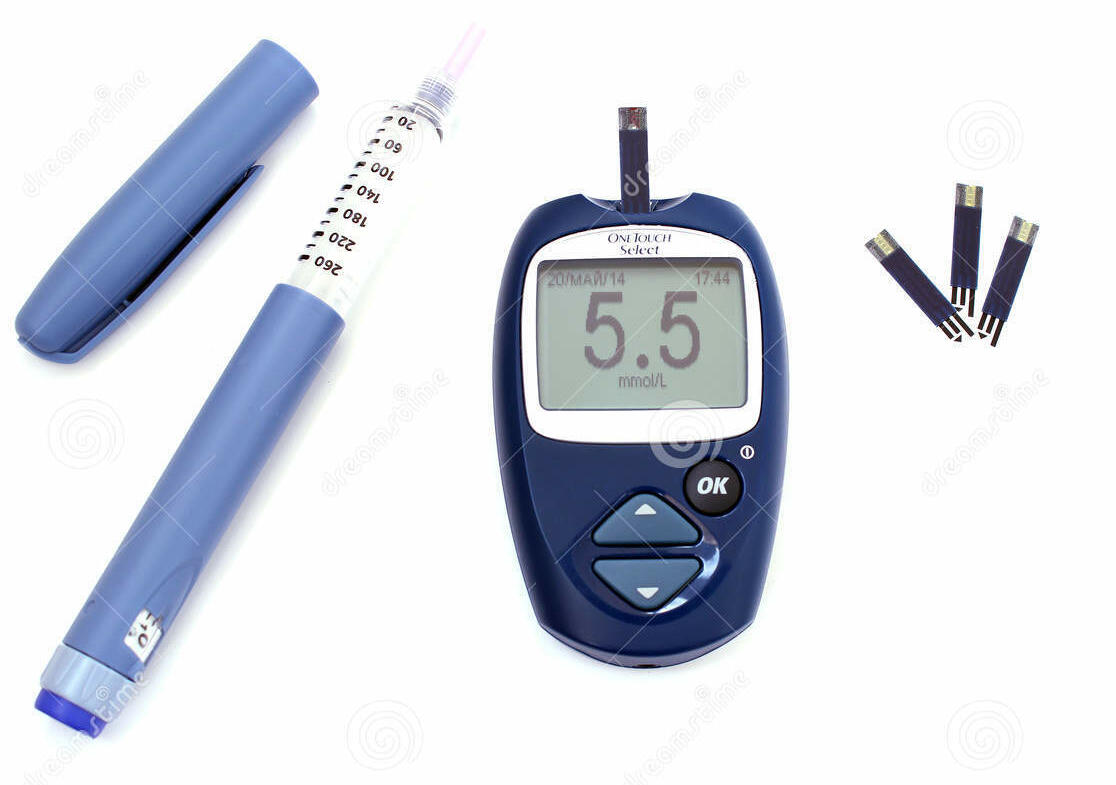
\includegraphics[width=0.5\textwidth]{images/glucometer.jpg}
        \caption{
         An image showing a modern insulin pen and glucometer \cite{penandglucometer}
        }
    \end{figure}
    This method of self-monitoring of blood glucose (SMBG) has significant drawbacks as blood is sampled intermittently, providing only short insights of glucose concentrations, whilst ignoring ongoing glucose fluctuations. With the idea of being able to monitor blood glucose at all times, Continuous Glucose Monitoring (CGM) devices were introduced that measure glucose concentrations at intervals (usually between 1-5 min), and then transmits/stores those values. Alongside the invention of the insulin pump, a device that allows programmable infusions of insulin over long, or short, periods of time, diabetic patients were given a much more reliable way of constantly monitoring and regulating their blood glucose levels.
    \begin{figure}[H]
      \centering
      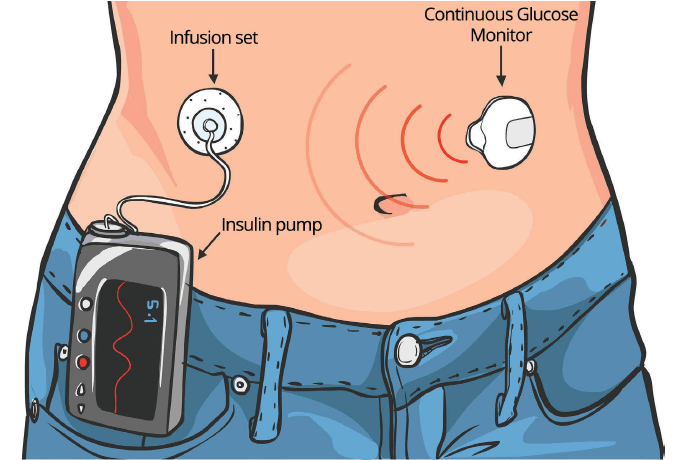
\includegraphics[width=0.5\textwidth]{images/CGMPump.png}
      \caption{
       A diagram showing the interaction between a CGM and insulin pump\cite{pumpandmonitor}
      }
    \end{figure}
    
    The creation of CGM devices also lead to a new capability - the ability to create blood glucose datasets by accessing the data stored in the CGM; datasets which are needed to train accurate Machine Learning (ML) models. It is clear that the capability to accurately predict when one might suffer a hyperglycemic, or hypoglycemic, episode would be invaluable to a T1DM patient, as it would allow them to behave proactively to prevent the episode from ever occurring, rather than the current reactionary method, which requires a hypo/hyperglycemic episode to be taking place before we can detect its presence. We name the amount of time into the future which we forecast the Prediction Horizon (PH). Current prediction horizons available to T1DM patients are very short, and thus don't give ample time for patients to react to predicted issues. Current CGM devices are capable of crude alarm systems that can inform patients if their BG levels are steeply dropping or rising, but once again this is just a reactionary measure. As such, much work has been done in applying ML techniques to improve the length of the PH to a length of hours instead of minutes, but as of yet no concrete solution to the problem has been found. This is due to a variety of reasons, such as the variability of a patient's BG level, due to day-to-day uncontrollable factors as mentioned earlier, as well as some other issues that will be discussed later when different approaches that have been experimented with to solve this very problem are explored.

	\subsection{Detail}
    \subsection{Machine Learning}
      Add section about papers / machine learning in general. Will consider whether to put ML here or later on.

      Machine learning is a field of Artificial Intelligence that focuses on learning through observing patterns in large quantities of past data, and iteratively improving accuracy at a given task \cite{whatisml}. In the context of T1DM, the large quantities of past data refer to the patient's blood glucose levels over a period of months (as well as other points of interest such as exercise undertaken / carbohydrate intake / insulin intake), whilst the task to improve at is predicting the BG levels of the patient for a specified PH. There is interest in the use of Artificial Neural Networks (ANN), a kind of Machine learning model that is able to learn very complex relationships between data \cite{whatisnn}. ANNs are based off of the functioning of the human brain, and are capable of modifying their structure to suit the task at hand. They consist of a number of nodes and a corresponding number of connections which link one node to another, where each connection has a weight which signals how strong the connection between the two nodes is. An ANN can consist of many layers with the first and last layers being known as the input and output layers respectively. Any layers inbetweeen the two are called hidden layers. Each node has an input into it, and in the final layer of the network, an output is given. At each node, every input is multiplied to its corresponding weight, and an activation function is applied to sum of these values to generate the output value to be passed to the next layer of the network. An activation function is a function that transforms the output in some way - for example the binary step activation function checks if the value is above a given threshold. If so, the node outputs 1, otherwise 0.
      \begin{figure}[H]
        \centering
        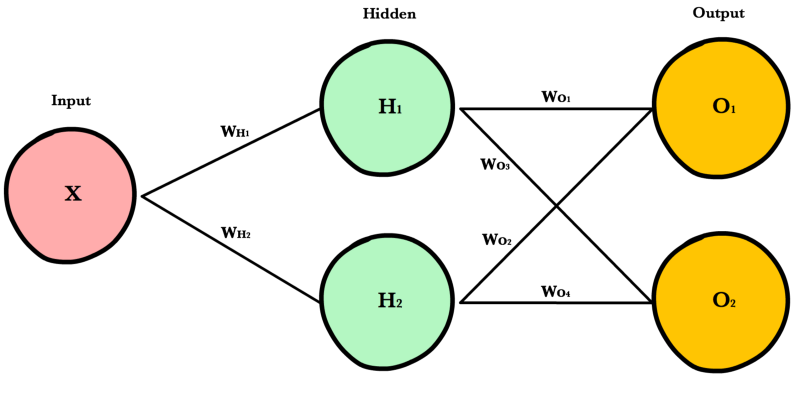
\includegraphics[width=0.5\textwidth]{images/basicNN.png}
        \caption{
         A diagram showing the nodes connections and weights of a simple ANN \cite{whatisnnimage}
        }
      \end{figure}
      In order for the NN to learn the task at hand, we define an error function between the actual output of a given input and the output generated by our network. This error function can be specified to suit the model as needed and it is common, in the case of blood glucose forecasting, to see an error function comparing the absolute difference between predicted blood glucose levels, and real recorded blood glucose levels. Through an iterative algorithm such as gradient descent \cite{whatisgd}, whereby we calculate the derivative of the error function and attempt to iteratively adjust the network weights to reach the minimum value of this function, the ANN can learn very complex relationships between the data input into it and the expected outputs. 
      \begin{figure}[H]
        \centering
        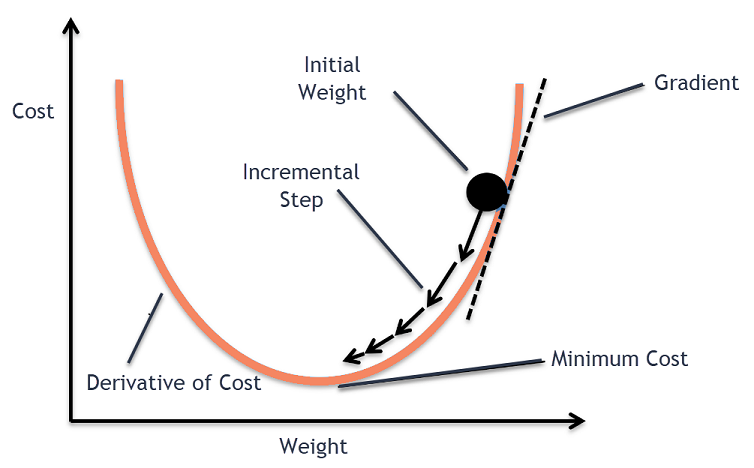
\includegraphics[width=0.5\textwidth]{images/gradientdescent.png}
        \caption{
         A visualisation of the gradient descent process\cite{whatisgdimage}
        }
      \end{figure}
      Much work has been done researching the applications of different kinds of ANN to blood glucose forecasting, as it was believed that not only would ANNs be able to provide very accurate predictions on future BG levels, but also would be able to solve the problem of inter-subject variability - by training a new network on each individual patient's BG data. 

      As will be seen below, when training neural networks, there is much debate amongst researchers about what to include and what not to include within the input parameters to the network. Some believe that just the CGM data is sufficient, claiming that the inclusion of other measures, such as carbohydrate intake, would simply increase variance and decrease model performance. This is sharply contrasted by researchers who have experimented with both complex and simple physiological models to try and model the effect that factors such as exercise and insulin intake will have on future glucose levels. There is much debate about the correlation between past glucose levels and future levels, with some using only the current blood glucose levels as an input to the model, and others using many past readings to inform future predictions. Whilst there is much diversity amongst the methods employed, unfortunately, the overarching theme from most ANN approaches is that they can be very accurate at shorter PH (~30 minutes), but that accuracy quickly drops off at larger PH (~6 hours).

      \subsection{Simple ANN Approaches}

      One such example of the application of NNs to the task of blood glucose prediction was by Pérez-Gandía et al.\cite{paper3}, who attempted to use a NN trained using only CGM data. The model considered the preceding 20 minutes of CGM data and attempted to predict BG levels at 3 different PHs of 15, 30 and 45 minutes. The accuracy of the model was measured using a number of different metrics. One such metric is the Root Mean Squared Error (RMSE) - a widely used metric for BG prediction models that takes the square root of the sum of the squares of all prediction errors. -Another the Prediction Delay (PD) - a metric that takes into account the delay between when certain features of the CGM data were seen in the original data and the predicted data (for instance the time gap between a peak appearing in the original and predicted data). When making a prediction, two different approaches were compared - a standard NN model that would make one prediction across the PH, and an AutoRegressive Model (ARM). In an ARM, the model makes the prediction one step at a time and uses a recursive algorithm to allow each prediction to inform subsequent predictions, trying to capture the relationships between previous and future BG levels more accurately. It was found that across the 15, 30 and 45 minute PHs there was a RMSE of ~10, 18, 27, mg/dL respectively. For upward trends in the data, there was a PD of 4, 9 and 14 minutes respectively, and for downward trends, a PD of 5, 15 and 26 minutes was seen. 


	\subsection{Summary}
            Lit review conclusions and summary, lead on to what work we are going to do

%%%%%%%%%%%%%%%%%% SECTION 3 %%%%%%%%%%%%%%%%%%
\section{Methods} % edit section heading as appropriate
    \subsection{Introduction}
        Briefly introduce the experiments we are going to perform, and the tools we are going to use to do so.
	
	\subsection{Detail}
        Tell story of the development of the models, from data processing to choices made in model hyperparameters / cleaning etc.
	
	\subsection{Summary}
        Provide a brief summary of development that leads on to results of the experiments performed.


%%%%%%%%%%%%%%%%%% SECTION 4 %%%%%%%%%%%%%%%%%%
\section{Results and discussion} % edit section heading as appropriate
    \subsection{Introduction}
        Briefly introduce results section, talk about metrics we are going to use etc.
	
	\subsection{Detail}
        Show different metrics and graphs e.g. table of RMSE across different time spans for different models, plots of metrics vs hyperparameter settings / regularised vs not regularised etc.
	
	\subsection{Summary}
        Provide a brief summary of the results seen and what they show us

% Add more sections if necessary


%%%%%%%%%%%%%%%%%% SECTION 5 %%%%%%%%%%%%%%%%%%
\section{Conclusions and future work} % edit section heading as appropriate
    \subsection{Conclusions}
        Talk generally about the parallels and differences seen from my approach vs the approaches studied in the literature review. Explain limitations of the task in reality.
	
	\subsection{Future work}
        Go into detail about how the model could be improved / what it would take to put such a model out into the real world via CGM/Pump.
    


%%%%%%%%%%%%%%%%%% REFERENCES %%%%%%%%%%%%%%%%%%
%\clearpage % uncomment to start on a new page if wanted
\printbibliography[title={References},heading=bibintoc] % a single list of references for the whole thesis



%%%%%%%%%%%%%%%%%% APPENDICES %%%%%%%%%%%%%%%%%%
\begin{uomappendix} 
    \section{Project outline}
    Project outline as submitted at the start of the project is a required appendix. Put here. 
    
    \section{Risk assessment}
    Risk assessment is a required appendix. Put here.

    %\section{Other appendices as necessary}
\end{uomappendix}


%%%%%%%%%%%%%%%%%% END MATTER %%%%%%%%%%%%%%%%%%
\end{document}